\documentclass{beamer}

%%%%%%%%%%%%%%%%%%%%%%%%%%%%%%%%%%{Sty}%%%%%%%%%%%%%%%%%%%%%%%%%%%%%%%%%%%%%%%%

% \usepackage{beamerthemeshadow}
\usepackage{graphicx}

\usepackage{tikz}
\usetikzlibrary{fadings}


% Math
\usepackage{amsmath,amsfonts,amssymb}
\usepackage{xfrac}


% Font
\usepackage[T1]{fontenc}
% \usepackage[garamond]{mathdesign}
\usepackage{garamondx}

% Color
\usepackage{xcolor}



%%%%%%%%%%%%%%%%%%%%%%%%%%%%%%%%%{Global}%%%%%%%%%%%%%%%%%%%%%%%%%%%%%%%%%%%%%%

% Author(s)
\newcommand{\presentationAuthorNameLong}{%
  Ali Bozorgzadeh \inst{1} \and Abas Ramiar \inst{2}}
\newcommand{\presentationAuthorNameShort}{A. Bozorgzadeh}
\newcommand{\presentationAuthorEmail}{%
  aliiiib95@gmail.com \inst{1} \\ aramiar@gmail.com \inst{2}}

% University/company
\newcommand{\presentationUniversityLong}{Babol Noshirvani University of Technology}
\newcommand{\presentationUniversityShort}{B.N.U.T}


% Title/subject
\newcommand{\presentationTitleLong}{Capacitive Deionization}
\newcommand{\presentationTitleShort}{Capacitive Deionization}
\newcommand{\presentationSubTitle}{A look at Numerical Studies}

% Misc.
\newcommand{\etal}{{\it et. al.}}

\newcommand{\gradient}{\noindent%
  
\begin{tikzpicture}
    % \fill[cyan,path fading=east] (0,1em) rectangle (\linewidth,1.5em);
    % \node at (.5\linewidth,0) {\bfseries #1};
    \fill[cyan,path fading=west, path fading=east] (0,-1em) rectangle (\linewidth,-1.5em);
  \end{tikzpicture}%
}

%% Nomenclature
% source: https://tex.stackexchange.com/a/147685/220469
\newcommand{\nomenclature}[2]{\item{\makebox[2cm]{#1\hfill} #2}}

%% Scientific notation
% source: https://tex.stackexchange.com/a/269848/220469
\newcommand{\expnumber}[2]{{#1}\mathrm{e}{#2}}

%% Bold face for vectors in math mode
\newcommand{\vect}[1]{\boldsymbol{#1}}

%% Custom Partial Derivative
\newcommand{\dd}[2]{\frac{\partial #1}{\partial #2}}

%% Partial Time Derivative
\newcommand{\ddt}[1]{\frac{\partial #1}{\partial t}}

%% Boxed display equations
\newcommand{\boxedeqn}[1]{
  \[\boxed{
    #1
  }\]
}



%%%%%%%%%%%%%%%%%%%%%%%%%%%%%%%{Config}%%%%%%%%%%%%%%%%%%%%%%%%%%%%%%%%%%%%%%%%%
% Set the global variables
\title[\presentationTitleShort]{\presentationTitleLong}
\subtitle{\presentationSubTitle}

%% \author[\presentationAuthorNameShort]{\presentationAuthorNameLong}

%% \institute[\presentationUniversityShort]{%
%%   \presentationUniversityLong \\ \medskip \texttt{aliiiib95@gmail.com}}
%% \date{\today}

%% \titlegraphic{%
%%   {\center
%%   \vspace{-2.5cm}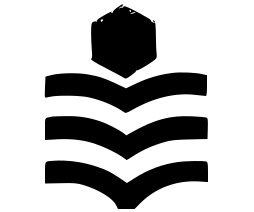
\includegraphics[height=1cm]{./logo.pdf}}} %You can modify the location of the logo by changing the command \vspace{}.

% \logo{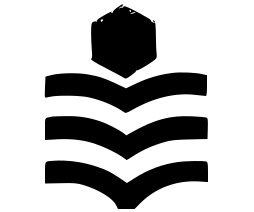
\includegraphics[height=1cm]{logo.pdf}}


%% Set beamer fonts
\usefonttheme{serif}

%% Dim out "inactive" elements
% source: https://tex.stackexchange.com/a/230467/220469
\setbeamercovered{transparent}
% NOTE: to make footnote only appear in the determined point
% use: \footnote<.(1)->

%% Remove footline navigation bar
%   \beamertemplatenavigationsymbolsempty
% Remove navigation bar but keep the frame numbering
\setbeamertemplate{navigation symbols}{%
  \usebeamerfont{footline}%
  \usebeamercolor[fg]{footline}%
  \insertsection \hspace{2cm}
  \hfill \insertframenumber/\inserttotalframenumber
}
\setbeamercolor{footline}{fg=gray}
%% \setbeamerfont{footline}{series=\bfseries}
\setbeamercolor{date in title}{fg=Brown}
\setbeamerfont{footnote}{size=\tiny}


%% Smaller itemize/enumerate font size
% source: https://tex.stackexchange.com/a/91582/220469
%% \setbeamertemplate{itemize/enumerate body begin}{\footnotesize}


%% Add section page
% source: https://tex.stackexchange.com/a/178803/220469
\AtBeginSection[]{
  \begin{frame}
    \vfill
    \centering
    \begin{beamercolorbox}[sep=8pt,center,shadow=true,rounded=true]{title}
      \usebeamerfont{title}\insertsectionhead\par%
    \end{beamercolorbox}
    \vfill
  \end{frame}
}

%% Reset footnote counter for each frame
% source: https://tex.stackexchange.com/a/530528/220469
\AtBeginEnvironment{frame}{\setcounter{footnote}{0}}

%% Center the title horizontally
% source: https://tex.stackexchange.com/a/329883/220469
\setbeamertemplate{frametitle}[default][center]



\begin{document}
%%%%%%%%%%%%%%%%%%%%%%%%%%%%%%%%{Document}%%%%%%%%%%%%%%%%%%%%%%%%%%%%%%%%%%%%%%

% ------------------------------------------------------------------------------
% Title frame
{
  % Disable numbering in the title frame
  % source: https://tex.stackexchange.com/a/18829/220469
  \setbeamertemplate{navigation symbols}{}
  \begin{frame}
    \maketitle
  \end{frame}
}


% ------------------------------------------------------------------------------
% Outline
\begin{frame}{Outline}
  %% \framesubtitle{my sub-title}
  \begin{itemize}
  \item A. Hemmatifar \etal -- 2015
  \item X. Shang \etal -- 2017
  \item Bieshuvel \etal -- 2010
  \item Salamat \etal -- 2020
  \end{itemize}
\end{frame}


%% % ------------------------------------------------------------------------------
%% % Shang
%% \section{X. Shang \etal -- 2017}
%% \begin{frame}
  \frametitle{Equations}
  \framesubtitle{Based on the amphoteric Donnan (\it{amph-D}) model}
  \begin{columns}
    \begin{column}{0.5\textwidth}
      % Concentration
      \[
      \frac{\partial \varepsilon_{ma} c}{\partial t}
      + \nabla \cdot \left( - D_{eff} \nabla{c}  \right)
      = \dot{S}
      \]

      % Source Term
      \[
      \dot{S}(\phi_s - \phi_e, c) = - \frac{\varepsilon_{mi}}{F}
      \frac{\partial c_{ions,\,mi}}{\partial t}
      \]

      % Current conservation
      \[
      \nabla \cdot (- \kappa_{eff} \nabla \phi_e) = \varepsilon_{mi} \dot{Q} + i_L
      \]

      % Salt concentration in flow channel
      \[
      \varepsilon_{FC} + \nabla{(\vec{v_s}) c}
      + \nabla{(- D_{eff,FC} \nabla{c})}
      \]
    \end{column}

    \begin{column}{0.5\textwidth}  %%<--- here

      % Charge Balance
      \[
      \rho_e - \rho_{mi} - \rho_{chem} = 0
      \]

      % Potential Balnace
      \[
      \phi_s - \phi_e = \Delta \phi_S + \Delta \phi_D
      \]

      \[
      \Delta \phi_S = \frac{F \rho_e}{\rho_{electrode} C_S}, \,
      \Delta \phi_D = \frac{\rho_mi}{2c}
      \]

      \[
      (c_{ions,\,mi})^2 = (\rho_{mi})^2 + (2 c F)^2
      \]
    \end{column}
  \end{columns}
\end{frame}

\begin{frame}
  \frametitle{Nomenclature}
  \tiny
  \begin{itemize}
    \nomenclature{$\varepsilon_{ma}$}{macro-porosity ($0.35$)}
    \nomenclature{$\varepsilon_{mi}$}{micro-porosity ($0.25$)}
    \nomenclature{$\varepsilon_{FC}$}{porosity of the flow channel spacer ($0.75$)}
    \nomenclature{$c$}{local salt concentration},
    \nomenclature{$c_{ions,\,mi}$}{ionic concentration in micro-pores}.
    \nomenclature{$\dot{S}$}{source/sink term}
    \nomenclature{$D_{eff}$}{effective salt diffusivity}\footnote{
    calculated based on porosity and bulk salt diffusivity, $D_0 = \expnumber{1.61}{-5}$ as $D_{eff} = D_0 \varepsilon^{1.5}$},
    \nomenclature{$D_{eff,FC}$}{effective salt diffusion coefficient in the flow
    \nomenclature{$F$}{Faraday Constant},
    \nomenclature{$\rho_e$}{electronic charge density},
    \nomenclature{$\rho_{mi}$}{ionic charge density},
    \nomenclature{$\rho_{chem}$}{surface immobile charge (4 $\mathrm{C/cm^3}$)},
    \nomenclature{$\Delta \phi_S$}{Stern Layer potential drop},
    \nomenclature{$\Delta \phi_D$}{Donnan Layer potential drop},
    \nomenclature{$\rho_{electrode}$}{electrode density (0.4664 $\mathrm{\sfrac{g}{cm^3}}$)},
    \nomenclature{$\kappa_{eff}$}{local effective
      ionic-conductivity}\footnote{It depends on the porosity and the
    corresponding bulk value: $\kappa_{eff} = \kappa_0\varepsilon^{1.5}$.
    According to Nernst-Einstein relation: $\kappa_0 = \sfrac{2 D_0 c F e}{k_B
      T}$},
    \nomenclature{$i_L$}{leakage current per unit electrode
      volume}\footnote{Due to parasitic faradaic reactions on the electrode}.
    \nomenclature{$\vec{v_s}$}{superficial velocity (assumed uniform)},
      channel}
  \end{itemize}
  \normalsize
\end{frame}

\begin{frame}
  \frametitle{Assumptions}
  \begin{itemize}
  \item Since the {\it\color{blue} direction of the current} is
    \textbf{perpendicular} to the {\it\color{blue} direction of the flow}, a
    \textbf{two dimensional} model is formulated for the continuous-flow
    operation scheme.
  \item In the model of \textbf{pulse-flow operation}, the effect of
    \textit{advection} can be {\color{red} neglected}, If we assume
    \begin{itemize}
    \item the event of pulsing happens \textbf{instantaneously}.
    \item This assumption {\it simplifies} the numerical implementation for
      pulse-flow operation and yeilds a {\color{red} one-dimensional}
      problem\footnote{Because the variation along the direction of the flow
      does not occur}.
    \end{itemize}
    \item Some other assumptins related to the faradaic reactions\dots
  \end{itemize}
\end{frame}

\begin{frame}
  \frametitle{Boundary and Initial Conditions}
  \begin{itemize}
  \item<1> {\bf Ionic flux} (excluding advective contributions) is set to zero at
    all surfaces except at flow-channel inlet.
  \item<2> {\bf Constant concentration} boundary condition at the flow-channel
    inlet.
  \item<3> In the {\it absence of flow}\footnote<.(1)->{For the one-dimensional model of
  pulse-flow operation} a {\bf null-flux} condition is imposed at the flow channel
    inlet. (?)
  \item<4> The {\bf total electronic current} at the {\it current collector
    surface} of the positive/negative electrode is constrained to the {\it total
    externally applied current}, while the {\bf total ionic current} is set to
    {\it zero} on these surfaces.
  \item<5> In all simulations we initialize the {\bf salt concentration} across
    the entire cell to the {\color{red} chosen in-fluent concentration}, and
    {\bf charge density} within the porous electrodes is initially set to
    {\color{red} zero}.
    \begin{itemize}
    \item From these initial conditions, initial cell voltage and ionic
      concentration inside micropores were calculated.
    \end{itemize}
  \end{itemize}
\end{frame}


%% ------------------------------------------------------------------------------
%% Hemmatifar
\section{A. Hemmatifar \etal -- 2015}

\begin{frame}
  \frametitle{Transport Equations}

  Let us begin with the general form of the
  mass transport equation (without reaction for species $i$)
  \[
  \frac{\partial c_i}{\partial t}
  + \nabla{\vect{j}}
  = \dot{S}
  \]
\end{frame}


\begin{frame}
  \frametitle{Equations}
  \framesubtitle{Based on the Improved Modified Donnan ({\it i-mD}) Model}
  \begin{columns}
    \begin{column}{0.5\textwidth}
      % Concentration
      \[
      \frac{\partial \varepsilon_{ma} c}{\partial t}
      + \nabla \cdot \left( - D_{eff} \nabla{c}  \right)
      = \dot{S}
      \]

      % Source Term
      \[
      \dot{S}(\phi_s - \phi_e, c) = - \frac{\varepsilon_{mi}}{F}
      \frac{\partial c_{ions,\,mi}}{\partial t}
      \]

      % Current conservation
      \[
      \nabla \cdot (- \kappa_{eff} \nabla \phi_e) = \varepsilon_{mi} \dot{Q} + i_L
      \]

      % Salt concentration in flow channel
      \[
      \varepsilon_{FC} + \nabla{(\vec{v_s}) c}
      + \nabla{(- D_{eff,FC} \nabla{c})}
      \]
    \end{column}

    \begin{column}{0.5\textwidth}  %%<--- here

      % Charge Balance
      \[
      \rho_e - \rho_{mi} - \rho_{chem} = 0
      \]

      % Potential Balnace
      \[
      \phi_s - \phi_e = \Delta \phi_S + \Delta \phi_D
      \]

      \[
      \Delta \phi_S = \frac{F \rho_e}{\rho_{electrode} C_S}, \,
      \Delta \phi_D = \frac{\rho_mi}{2c}
      \]

      \[
      (c_{ions,\,mi})^2 = (\rho_{mi})^2 + (2 c F)^2
      \]
    \end{column}
  \end{columns}
\end{frame}


% ------------------------------------------------------------------------------
% Biesheuvel
%% \section{}

\end{document}
